\documentclass[12pt,a4paper]{article}
\usepackage[utf8]{vietnam}
\usepackage{amsmath,amssymb}
\usepackage{tabularx}
\usepackage{tikz}
\usetikzlibrary{calc,angles,quotes,arrows.meta,patterns}
\usepackage{xcolor}
\usepackage{enumitem}
\usepackage{fancyhdr}
\usepackage{graphicx}
\usepackage[top=1.2cm, bottom=1.2cm, left=1.5cm, right=1.5cm]{geometry}
\usepackage[dethi]{ex_test}
\SAOPTN{widthSA=2.6,heightSA=0.62}

\setlength{\headheight}{15pt}
\setlength{\parskip}{0pt}

\pagestyle{fancy}
\fancyhf{}
\rhead{\textit{Môn Toán 6 -- Đề số 14}}
\lhead{\textit{Bộ đề ôn tập Giữa học kì I}}
\cfoot{\thepage}

\begin{document}

% --- KHUNG TIÊU ĐỀ ĐỀ THI ---
\noindent
\begin{tabularx}{\linewidth}{X r}
\textbf{TRƯỜNG THCS: \dotfill} & \textbf{ĐỀ KIỂM TRA ĐỊNH KỲ GIỮA HỌC KỲ I} \\
\textbf{Họ và tên: \dotfill} & \textbf{NĂM HỌC 2026 -- 2027} \\
\textbf{Lớp: \dotfill \quad SBD: \dotfill} & \textbf{Môn: TOÁN 6} \\
\hline
\end{tabularx}
\vspace{2mm}

\begin{center}
  \textbf{\large ĐỀ ÔN TẬP GIỮA HỌC KỲ I -- ĐỀ SỐ 14}\\
  \textit{Thời gian làm bài: 90 phút (Không kể thời gian phát đề)}
\end{center}
\vspace{1mm}

% --- PHẦN I ---
\noindent\textbf{\large PHẦN I. CÂU TRẮC NGHIỆM NHIỀU PHƯƠNG ÁN LỰA CHỌN (3,0 điểm)}

\textit{Thí sinh trả lời từ câu 1 đến câu 12. Mỗi câu hỏi thí sinh chỉ chọn một phương án duy nhất.}

\vspace{1mm}
\begin{ex}
$\text{ƯCLN}(18, 60)$ là:
\choice
{\True 6}
{12}
{18}
{30}
\end{ex}

\begin{ex}
Hai đường chéo của hình chữ nhật $MNPQ$ là:
\begin{center}
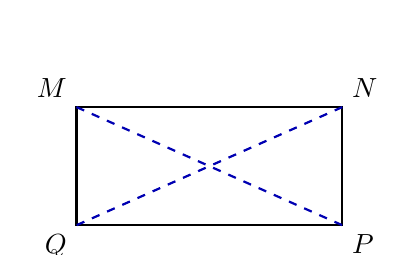
\begin{tikzpicture}[scale=0.75, baseline=(current bounding box.center)]
  \coordinate (M) at (0,2);
  \coordinate (N) at (4.5,2);
  \coordinate (P) at (4.5,0);
  \coordinate (Q) at (0,0);
  \draw[thick] (M) -- (N) -- (P) -- (Q) -- cycle;
  \draw[thick, dashed, blue!70!black] (M) -- (P);
  \draw[thick, dashed, blue!70!black] (N) -- (Q);
  \node[above left] at (M) {$M$};
  \node[above right] at (N) {$N$};
  \node[below right] at (P) {$P$};
  \node[below left] at (Q) {$Q$};
\end{tikzpicture}
\end{center}
\choice
{$MN$ và $QP$}
{\True $MP$ và $NQ$}
{$MQ$ và $NP$}
{$MN$ và $MQ$}
\end{ex}

\begin{ex}
Trong phép chia một số tự nhiên cho 4, số dư có thể là:
\choice
{1; 2; 3}
{0; 1; 2; 3; 4}
{\True 0; 1; 2; 3}
{0}
\end{ex}

\begin{ex}
Số nào sau đây chia hết cho cả 2 và 5?
\choice
{\True 1150}
{1155}
{5311}
{3536}
\end{ex}

\begin{ex}
Hình nào trong các hình sau có hai cạnh đối song song và hai đường chéo bằng nhau?
\choice
{Hình bình hành}
{\True Hình thang cân}
{Hình thoi}
{Hình tam giác đều}
\end{ex}

\begin{ex}
Cho tập hợp $A = \{0; 2; 4; a; b\}$. Khẳng định nào dưới đây là sai?
\choice
{\True $5 \in A$}
{$a \in A$}
{$0 \in A$}
{$1 \notin A$}
\end{ex}

\begin{ex}
Số nào sau đây là ước của 60?
\choice
{16}
{18}
{\True 20}
{22}
\end{ex}

\begin{ex}
Trong các số sau, số nào là bội của 4?
\choice
{1}
{2}
{\True 8}
{15}
\end{ex}

\begin{ex}
Trong các hình ảnh dưới đây, hình ảnh nào có dạng hình tam giác đều?
\begin{center}
\includegraphics[width=0.88\linewidth]{crops/test_p54_xref3332.jpeg}
\end{center}
\choice
{Hình 1}
{Hình 2}
{Hình 3}
{\True Hình 4}
\end{ex}

\begin{ex}
Khẳng định nào sau đây là khẳng định đúng về hình chữ nhật?
\choice
{Bốn cạnh bằng nhau}
{\True Hai đường chéo bằng nhau và cắt nhau tại trung điểm mỗi đường}
{Hai đường chéo vuông góc với nhau}
{Chu vi hình chữ nhật là tích của chiều dài và chiều rộng}
\end{ex}

\begin{ex}
Cho $x$ là số tự nhiên thỏa mãn $10^7 < x < 10^8$. Số $x$ có:
\choice
{9 chữ số}
{\True 8 chữ số}
{7 chữ số}
{10 chữ số}
\end{ex}

\begin{ex}
Hình chữ nhật có chiều dài $60\text{ dm}$ và chiều rộng $4\text{ m}$ thì diện tích là:
\choice
{\True $24\text{ m}^2$}
{$240\text{ dm}^2$}
{$200\text{ dm}^2$}
{$128\text{ dm}^2$}
\end{ex}


\vspace{1mm}
\noindent\textbf{BẢNG TRẢ LỜI TRẮC NGHIỆM PHẦN I:}
\begin{center}
\begin{tabular}{|c|c|c|c|c|c|c|c|c|c|c|c|c|}
\hline
\textbf{Câu} & \textbf{1} & \textbf{2} & \textbf{3} & \textbf{4} & \textbf{5} & \textbf{6} & \textbf{7} & \textbf{8} & \textbf{9} & \textbf{10} & \textbf{11} & \textbf{12} \\
\hline
\textbf{Chọn} & \rule{0pt}{0.65cm} & & & & & & & & & & & \\
\hline
\end{tabular}
\end{center}
\vspace{2mm}

\setcounter{ex}{0}
\noindent\textbf{\large PHẦN II. CÂU TRẮC NGHIỆM ĐÚNG SAI (2,0 điểm)}

\textit{Thí sinh trả lời câu 1 và câu 2. Trong mỗi ý a), b), c), d) ở mỗi câu, thí sinh chọn đúng hoặc sai.}

\vspace{1mm}
\begin{ex}
Cho các hình sau: hình tam giác đều, hình vuông, hình lục giác đều, hình chữ nhật, hình thoi, hình bình hành, hình thang cân. Xét tính đúng sai của các mệnh đề sau:
\choiceTF
{\True Hình tam giác đều, hình vuông, hình lục giác đều có tất cả các cạnh bằng nhau}
{\True Có 2 hình có hai đường chéo vuông góc với nhau}
{\True Có 3 hình hai cạnh đối song song và các đường chéo bằng nhau}
{Hình lục giác có độ dài đường chéo gấp đôi độ dài cạnh}
\end{ex}

\begin{ex}
Cho ba số $A = 24$, $B = 36$ và $C = 60$. Xét tính đúng sai của các mệnh đề sau:
\choiceTF
{\True Số 12 là một ước chung của ba số $A, B, C$}
{\True Phân tích số 24 ra thừa số nguyên tố ta được $2^3 \cdot 3$}
{Ước chung lớn nhất của hai số $A$ và $B$ là 6}
{\True Bội chung nhỏ nhất của hai số $A$ và $B$ là 72}
\end{ex}


\noindent\textbf{BẢNG TRẢ LỜI PHẦN II:}
\begin{center}
\begin{tabular}{|c|c|c|c|c||c|c|c|c|c|}
\hline
\textbf{Câu 1} & \textbf{a)} & \textbf{b)} & \textbf{c)} & \textbf{d)} & \textbf{Câu 2} & \textbf{a)} & \textbf{b)} & \textbf{c)} & \textbf{d)} \\
\hline
\textbf{Đ/S} & \rule{0pt}{0.6cm} & & & & \textbf{Đ/S} & & & & \\
\hline
\end{tabular}
\end{center}
\vspace{2mm}

\setcounter{ex}{0}
\noindent\textbf{\large PHẦN III. CÂU HỎI TRẢ LỜI NGẮN (2,0 điểm)}

\textit{Thí sinh trả lời câu 1 và câu 2. Điền kết quả số vào ô trống tương ứng.}

\vspace{1mm}
\begin{ex}
Cho hình thoi $ABCD$ có cạnh $5\text{ cm}$. Chu vi của hình thoi $ABCD$ là bao nhiêu centimét? \shortans{20}
\end{ex}

\begin{ex}
Tìm số tự nhiên $x$ lớn nhất thỏa mãn $30 \ \vdots \ x$ và $45 \ \vdots \ x$? \shortans{15}
\end{ex}


\setcounter{ex}{0}
\noindent\textbf{\large PHẦN IV. TỰ LUẬN (3,0 điểm)}

\textit{Thí sinh trình bày chi tiết lời giải vào giấy làm bài.}

\vspace{1mm}
\begin{ex} (2,0 điểm)
Thực hiện phép tính (tính nhanh nếu có):
\begin{enumerate}[label=\textbf{\alph*)}, leftmargin=0.8cm, itemsep=2pt]
\item (0,5 điểm) $115 + 300 + 585$
\item (0,5 điểm) $6^2 \cdot 25 + 4 \cdot 9 \cdot 75 - 25^0$
\item (0,5 điểm) $2025 \cdot 79 + 2025 \cdot 21$
\item (0,5 điểm) $10^2 - [60 : (5^6 : 5^4 - 3 \cdot 5)]$
\end{enumerate}
\end{ex}
\vspace{1.5mm}

\begin{ex} (1,5 điểm)
Tìm số tự nhiên $x$, biết:
\begin{enumerate}[label=\textbf{\alph*)}, leftmargin=0.8cm, itemsep=2pt]
\item (0,25 điểm) $x + 24 = 60$
\item (0,25 điểm) $3(x - 5) = 21$
\item (0,5 điểm) $3 \cdot 2^x + 12 = 36$
\item (0,5 điểm) $150 - 2(x + 1) = 70$
\end{enumerate}
\end{ex}
\vspace{1.5mm}

\begin{ex} (1,0 điểm)
Bạn An đi nhà sách mua 5 cây bút bi cùng loại và 6 quyển tập cùng loại. Biết giá tiền một quyển tập là $10\,000$ đồng. Bạn đưa chị thu ngân tờ $200\,000$ đồng và được chị trả lại $125\,000$ đồng. Hỏi giá tiền của 1 cây bút mà bạn An đã mua là bao nhiêu?
\begin{enumerate}[label=\textbf{\alph*)}, leftmargin=0.8cm, itemsep=2pt]
\item (1,0 điểm) Tính giá tiền của 1 cây bút bi.
\end{enumerate}
\end{ex}
\vspace{1.5mm}

\begin{ex} (0,5 điểm)
Cho $S = 3 + 3^2 + 3^3 + 3^4 + \dots + 3^{99} + 3^{100}$. Hỏi $S$ có chia hết cho 12 không? Vì sao?
\begin{enumerate}[label=\textbf{\alph*)}, leftmargin=0.8cm, itemsep=2pt]
\item (0,5 điểm) Chứng minh $S \ \vdots \ 12$.
\end{enumerate}
\end{ex}
\vspace{1.5mm}


\begin{center}
\rule{4cm}{0.4pt}\\
\textit{--- HẾT ---}
\end{center}
\end{document}
